% ...........................................................................
%                  E L L I P T I S C H E  K U R V E N
% ~~~~~~~~~~~~~~~~~~~~~~~~~~~~~~~~~~~~~~~~~~~~~~~~~~~~~~~~~~~~~~~~~~~~~~~~~~~

\newpage
\section{Elliptische Kurven}
\index{Elliptische Kurven}
\hypertarget{ellcurve}{}
(Filipovics B. / B"uger M. / Esslinger B. / Oyono R., April 2000, Updates: Dez. 2001, Juni 2002, M"arz 2003)

\subsection{Elliptische Kurven --- ein effizienter Ersatz f"ur RSA?} \label{ECAlternative}

In vielen Bereichen sind Sicherheit und Effizienz von Daten"ubertragungen von gro"ser
Wichtigkeit. Viele Anwendungen verwenden den RSA-Algorithmus als asymmetrisches Verschl"usselungsverfahren.

Solange die verwendeten Schl"ussel hinreichend lang sind, bestehen zur Zeit keinerlei Bedenken gegen die
Sicherheit des RSA. Allerdings hat die Entwicklung der Rechnerleistungen in der vergangenen Jahren dazu
gef"uhrt, dass die ben"otigten Schl"ussell"angen mehrfach angehoben werden mussten (vergleiche Kapitel \ref{SecurityRSA}).
Da die meisten Chips auf Smartcards\index{Smartcard} nicht in der Lage sind, l"angere Schl"ussel als
1024 bit zu verarbeiten, hat man Bedarf f"ur Alternativen zum RSA. Elliptische Kurven
k"onnen eine solche Alternative bieten.

Die Effizienz eines kryptographischen Algorithmus h"angt wesentlich von der ben"otigten \linebreak[4]Schl"ussell"ange
und dem Rechenaufwand ab, die notwendig sind, um ein vorgeschriebenes Sicherheitsniveau zu erreichen.
Der entscheidende Vorteil Elliptischer Kurven im Vergleich zum RSA-Algorithmus liegt in der Tatsache,
dass die ben"otigten Schl"ussell"angen erheblich k"urzer sind. 

Setzt man den Trend, dass sich die
Leistung der verf"ugbaren Rechner im Schnitt alle 18 Monate verdoppelt (Gesetz von Moore\index{Gesetz von Moore}), in die Zukunft
fort, so kann man von einer Entwicklung der ben"otigten Schl"ussell"angen
wie in Abbildung~\ref{RSAKeylength} ausgehen
(Quelle: Arjen Lenstra und Eric Verheul: 
\href{http://cryptosavvy.com/table.htm}{\texttt{http://cryptosavvy.com/table.htm}}).

% -> Figur 1
\begin{figure}[h]
\begin{center}
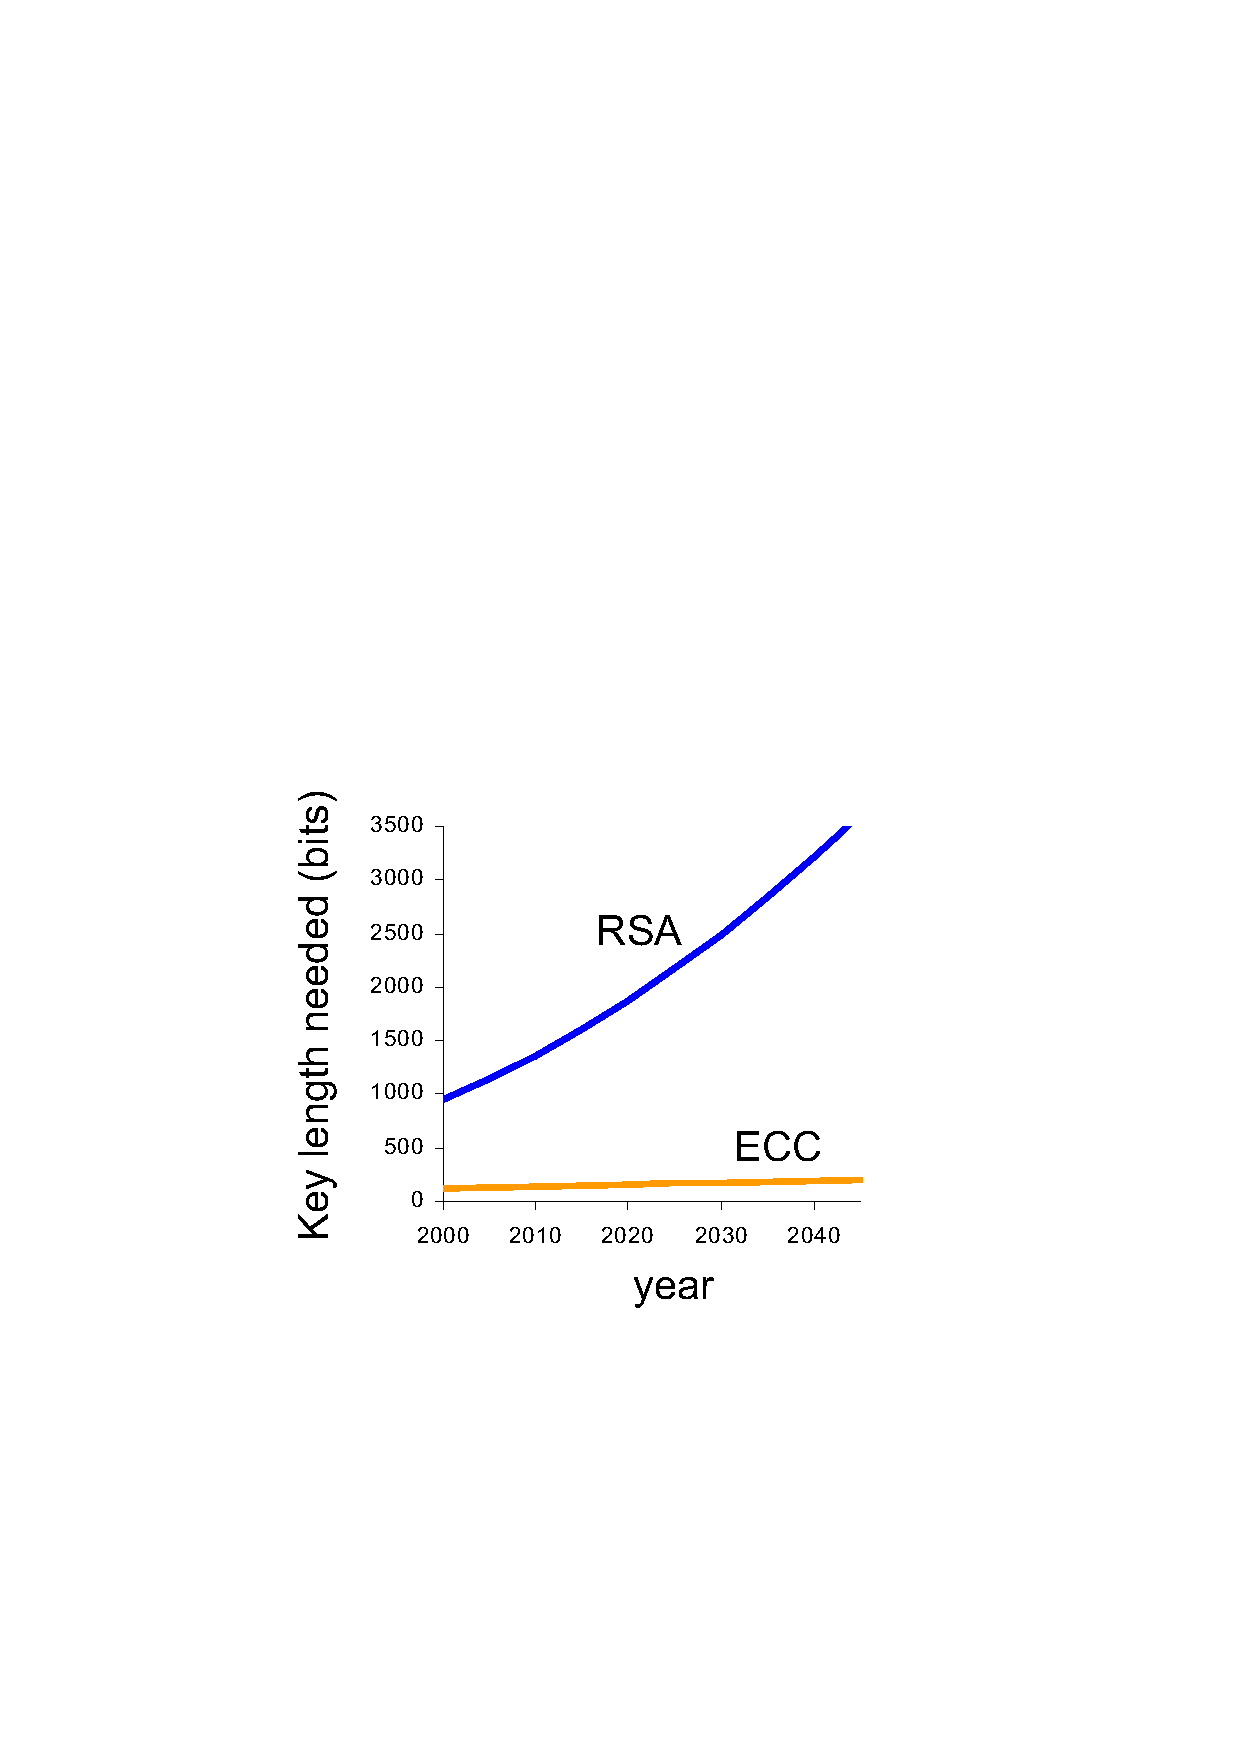
\includegraphics[scale=0.75]{figures/RSAKeylength}
\caption{Prognose f"ur die Entwicklung der als sicher betrachteten
  Schl"ussell"angen f"ur RSA und Elliptische Kurven\vspace{1ex}} 
\label{RSAKeylength}
\end{center}
\vskip -30 pt
\end{figure}

\newpage

Bei der digitalen Signatur muss man differenzieren: f"ur die {\em
  Erstellung} einer digitalen Signatur ben"otigen auf Elliptischen
Kurven basierende Verfahren im Vergleich zu RSA nur gut ein Zehntel des
Rechenaufwandes (66 zu 515 Multiplikationen). Siehe hierzu
Abbildung~\ref{ThousandBitMultiplications} (Quelle: Dr. J.  Merkle,
Elliptic Curve Cryptography Workshop, 2001). Betrachtet man die f"ur eine
{\em Verifikation} durchzuf"uhrenden Rechenschritte, dreht sich dieses Bild
jedoch zu Gunsten von RSA um. Der Grund liegt darin, dass es bei Verwendung
des RSA m"oglich ist, einen sehr kurzen "offentlichen Schl"ussel zu
w"ahlen, solange der private Schl"ussel nur hinreichend lang ist.

% -> Figur 2
\begin{figure}[h]
\vskip -40 pt
\begin{center}
\vspace{1.5cm}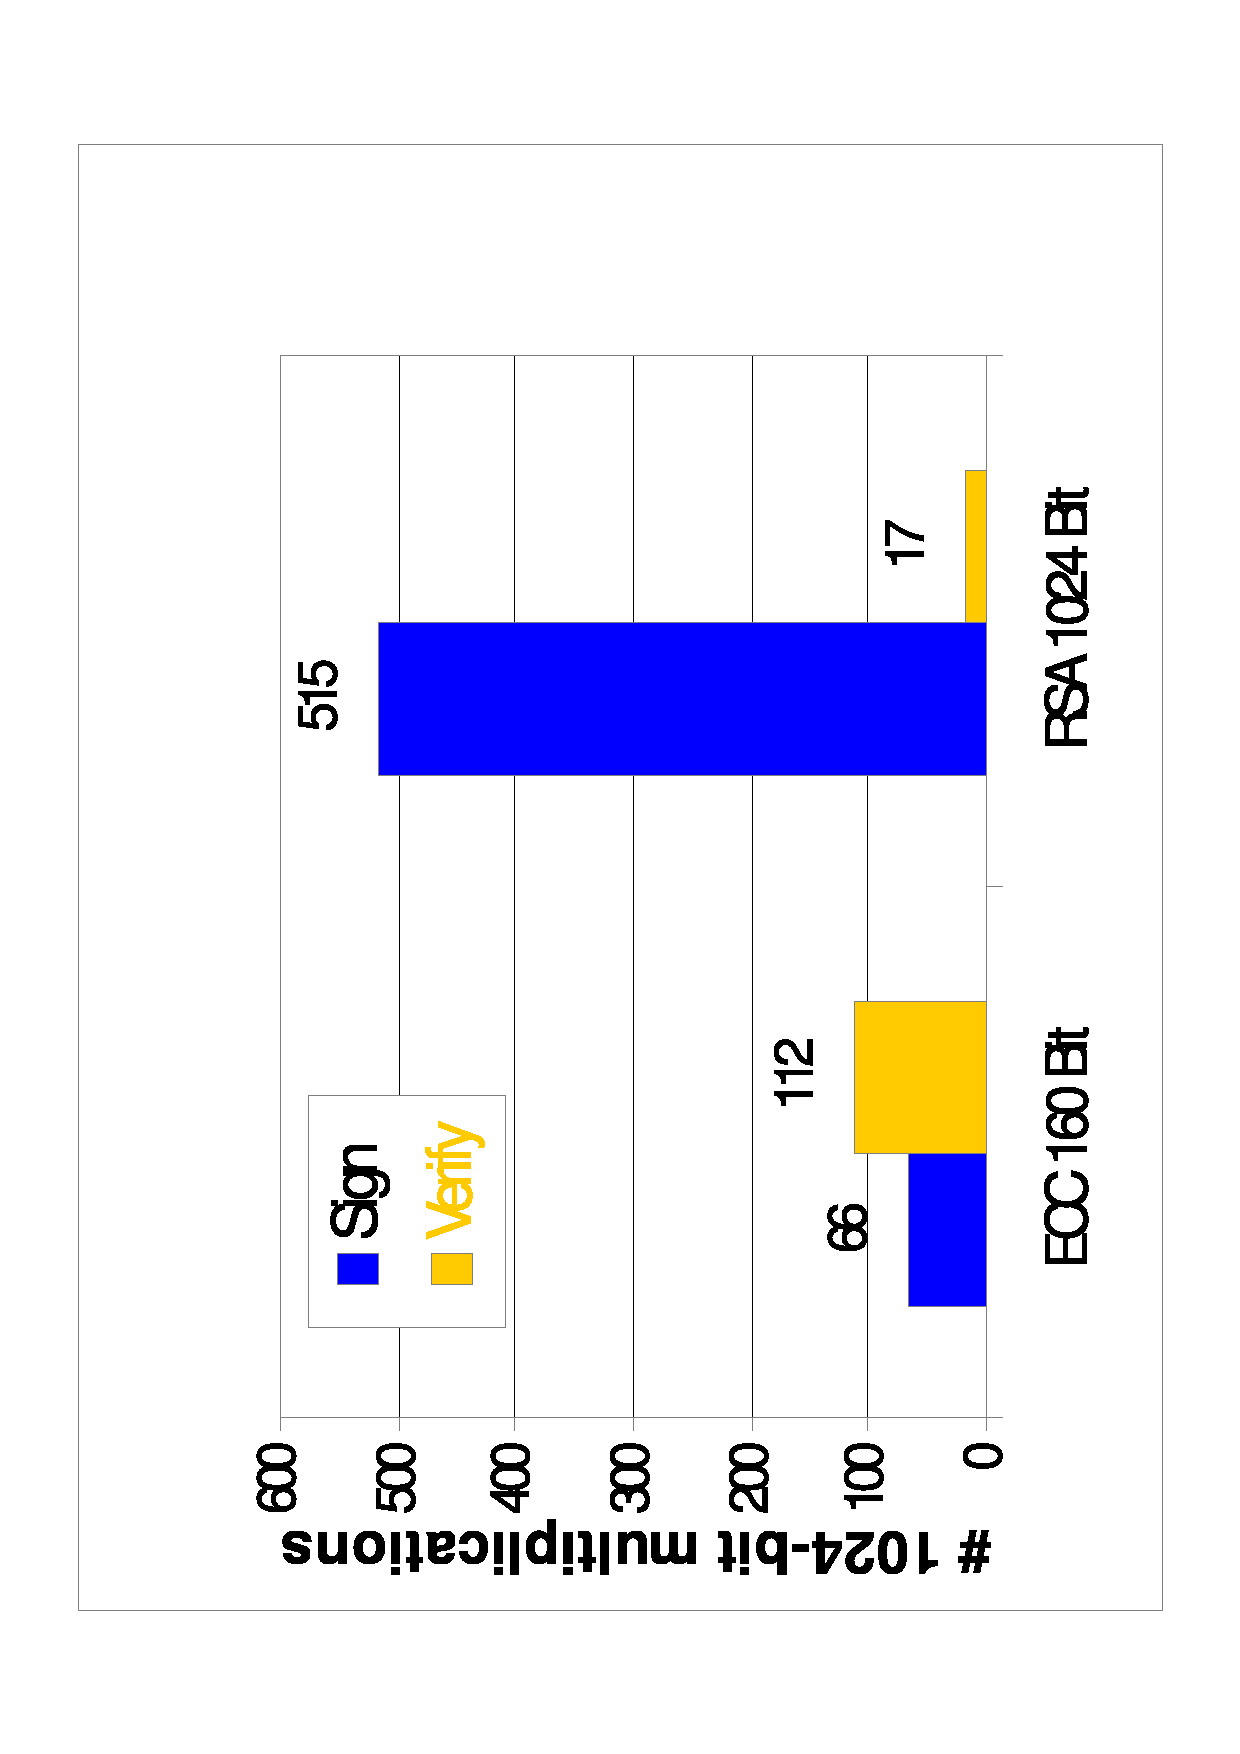
\includegraphics[scale=0.75]{figures/ThousandBitMultiplications}
\caption{Gegen"uberstellung des Aufwands der Operationen Signieren und Verifizieren bei
  RSA und Elliptischen Kurven} 
\label{ThousandBitMultiplications}
\end{center}
\vskip -10 pt
\end{figure}

Da bei Smartcard-basierten Systemen stets der lange private Schl"ussel auf der Karte gespeichert werden
muss und die Erstellung der digitalen Signatur, nicht aber die Verifikation, auf der Karte stattfindet, treten hier deutlich
die Vorteile Elliptischer Kurven zu Tage. 
\par
\smallskip
Das gr"o"ste Problem bei der Implementierung von Verfahren, die auf Elliptischen Kurven beruhen, ist bislang die
mangelnde {\em Standardisierung\index{Standardisierung}}. Es gibt nur eine RSA-Implementierung, aber viele Arten, Elliptische Kurven einzusetzen.
So k"onnen verschiedene Zahlk"orper zugrunde gelegt, eine Vielzahl von (Elliptischen) Kurven --- durch
6 Parameter beschrieben --- eingesetzt und unterschiedliche Darstellungen der Kurvenpunkte verwendet werden.
Jede Wahl hat ihre Vorz"uge, so dass f"ur jede Anwendung eine andere Implementierung optimal sein kann. Dies
hat jedoch zur Konsequenz, dass Systeme, die auf Elliptischen Kurven beruhen, oftmals nicht interoperabel
sind. Um mit einer beliebigen auf Elliptischen Kurven basierenden Anwendung kommunizieren zu k"onnen, m"usste man
eine Vielzahl von Implementierungen vorhalten, was den Effizienzvorteil gegen"uber der Verwendung von RSA
zunichte macht.

Deshalb bem"uhen sich internationale Organisationen hierzu um Standardisierung. Zu erw"ahnen sind
Initiativen von IEEE (P1363), ASC (ANSI X9.62, X9.63), IOS/IEC sowie von RSA Laboratories\index{RSA Laboratories} und Certicom\index{Certicom}. Im
Gegensatz zur IEEE, die bisher nur eine Beschreibung der verschiedenen Implementierungen vorgenommen hat,
hat die ASC konkret 10 Kurven ausgew"ahlt und empfiehlt deren Verwendung. Der Vorteil des ASC-Ansatzes ist,
dass ein einziges Byte ausreicht, um die verwendete Kurve zu spezifizieren. Zur Zeit ist jedoch nicht
absehbar, ob es der ASC gelingen wird, einen de-facto-Standard durchzusetzen.

Obwohl aktuell kein Handlungsbedarf besteht, laufende RSA-Anwendungen umzustellen, sollte man bei der
Neuimplementierung ernsthaft den Einsatz von Verfahren erw"agen, die auf Elliptischen Kurven basieren.
Dies gilt insbesondere, wenn es sich um Anwendungen im Finanzsektor handelt, die noch
nach 2005 operativ sein sollen.



\subsection{Elliptische Kurven --- Historisches}

Auf dem Gebiet der Elliptischen Kurven wird seit "uber 100 Jahren geforscht. Im Laufe der Zeit hat man
viele weitl"aufige und mathematisch tiefgr"undige Resultate im Zusammenhang mit Elliptischen Kurven gefunden
und ver"offentlicht. Ein Mathematiker w"urde sagen, dass die Elliptischen Kurven
(bzw.\ die dahinterstehende Mathematik) gut verstanden sind. Urspr"unglich war diese Forschung reine
Mathematik, das hei"st Elliptische Kurven wurden zum Beispiel in den mathematischen Teilgebieten
Zahlentheorie und algebraische Geometrie untersucht, die allgemein sehr abstrakt sind. Auch in der
nahen Vergangenheit spielten Elliptische Kurven eine bedeutende Rolle in der reinen Mathematik. In den
Jahren 1993 und 1994 ver"offentlichte Andrew Wiles\index{Wiles} mathematische Arbeiten, die weit "uber das Fachpublikum
hinaus auf gro"se Begeisterung gesto"sen sind. In diesen Arbeiten bewies er die Richtigkeit einer --- in
den sechziger Jahren des 20. Jahrhunderts von zwei Japanern aufgestellten --- Vermutung. Dabei geht es
kurz und grob gesagt um den Zusammenhang zwischen Elliptischen Kurven und sogenannten Modulformen.
Das f"ur die meisten eigentlich Interessante daran ist, dass Wiles mit seinen Arbeiten auch den ber"uhmten
zweiten Satz von Fermat\index{Fermat!letzter Satz} bewiesen hat. Dieser Satz hatte sich seit Jahrhunderten
(Fermat\index{Fermat} lebte von 1601 bis 1665) einem strengen Beweis durch die Mathematik entzogen. Dementsprechend
gro"s war die Resonanz auf den Beweis durch Wiles. In der Formulierung von Fermat lautet der nach ihm
benannte Satz so (Fermat hat folgende Worte an den Rand eines Buches geschrieben):

\begin{quote} {\em
Cubum autem in duos cubos, aut quadratoquadratum in duos quadratoquadratos, et
generaliter nullam in infinitum ultra quadratum potestatem in duos ejusdem nominis
fas est dividere: cujus rei demonstrationem mirabilem sane detexi. Hanc marginis
exiguitas non caperet.
} \end{quote}

Frei "ubersetzt und mit der Schreibweise der heutigen Mathematik bedeutet dies: \\
Es gibt keine positiven ganzen Zahlen $x, y$ und $z$ gr"o"ser als Null, so dass
$x^n + y^n = z^n$ f"ur $n>2$ gilt.
Ich habe einen bemerkenswerten Beweis f"ur diese Tatsache gefunden, aber es ist
nicht genug Platz am Rand [des Buches], um ihn niederzuschreiben.

Dies ist schon bemerkenswert: Eine relativ einfach zu verstehende Aussage
(gemeint ist Fermats zweiter Satz) konnte erst nach so langer Zeit bewiesen werden, obwohl
Fermat selber angab, schon einen Beweis gefunden zu haben.
Im "ubrigen ist der Beweis von Wiles sehr umfangreich (alle im Zusammenhang mit dem Beweis
stehenden Ver"offentlichungen von Wiles ergeben schon ein eigenes Buch). Man sollte sich daher
im klaren sein, dass die Elliptischen Kurven im allgemeinen sehr tiefgreifende Mathematik ber"uhren.

Soweit zur Rolle der Elliptischen Kurven in der reinen Mathematik. Im Jahr 1985 haben Neal Koblitz
und Victor Miller unabh"angig voneinander vorgeschlagen, Elliptische Kurven in der Kryptographie
einzusetzen. Damit haben die Elliptischen Kurven auch eine ganz konkrete praktische Anwendung gefunden.
Ein weiteres interessantes Einsatzgebiet f"ur Elliptische Kurven ist die Faktorisierung von ganzen Zahlen
(auf der \index{Komplexit"at} Schwierigkeit/Komplexit"at, die Primfaktoren einer sehr gro"sen Zahl zu finden, beruht
zum Beispiel das RSA-Kryptosystem). In diesem Bereich werden seit 1987 (eine Arbeit von H.W. Lenstra)
auf Elliptischen Kurven basierende Verfahren untersucht und zum Teil eingesetzt. Es gibt auch
Primzahltests\index{Primzahltest}, die auf Elliptischen Kurven basieren.

Elliptische Kurven werden in den verschiedenen Gebieten unterschiedlich eingesetzt.
Verschl"usselungsverfahren auf Basis von Elliptischen Kurven beruhen auf der
Schwierigkeit eines als Elliptische Kurven Diskreter Logarithmus bekannten Problems.
Die Faktorisierung von ganzen Zahlen macht sich die Tatsache zunutze, dass man f"ur eine nat"urliche,
aus mehreren Primzahlen zusammengesetzte Zahl $n$ sehr viele verschiedene Elliptische
Kurven erzeugen kann; diese Kurven sind dann allerdings f"ur zusammengesetzte $n$ keine
Gruppen. \hyperlink{faktell}{N"aheres dazu findet sich unter Faktorisieren mit Elliptischen Kurven.}

% ----------------------------------------------------------------------------------------------------------------
\subsection{Elliptische Kurven --- Mathematische Grundlagen}

In diesem Abschnitt erhalten Sie Informationen "uber
\index{Gruppen} {\em Gruppen} und \index{K""orper} {\em K"orper}.

\subsubsection{Gruppen}

Da der Begriff der {\em Gruppe} umgangssprachlich anders als in der Mathematik eingesetzt wird, soll der
Vollst"andigkeit halber an dieser Stelle die wesentliche Aussage der formalen Definition einer Gruppe
kurz eingef"uhrt werden:
\begin{itemize}
   \item Eine Gruppe ist eine nichtleere Menge $G$ mit einer Verkn"upfung $+$ . Die Menge $G$ ist unter der
         Verkn"upfung $+$ abgeschlossen. Egal welche beiden Elemente $a, b$ aus $G$ miteinander verkn"upft
          werden, so ist das Resultat der Verkn"upfung ein Element aus $G$ (also $a+b=c$, und $c$ liegt in $G$).
   \item F"ur alle Elemente $a, b$ und $c$ aus $G$ gilt: $(a+b)+c = a+(b+c)$.
   \item Es gibt ein Element $e$ in $G$, das sich bez"uglich der Verkn"upfung $+$ neutral verh"alt. Es gilt also f"ur alle $a$ aus der Menge $G:$ $~a+e = e+a = a.$
   \item Zu jedem Element $a$ aus $G$ gibt es ein sogenanntes inverses Element $-a$
         ($-a$ liegt auch in $G$), so dass gilt: $a+(-a) = (-a)+a = e$.
\end{itemize}
Gilt zus"atzlich noch f"ur alle $a, b$ aus $G$, dass $a+b = b+a$, so nennt man die Gruppe eine {\em abelsche} Gruppe.
Eine mit $+$ bezeichnete Verkn"upfung deutet auf eine {\em additive} Gruppe hin;
schreibt man die Verkn"upfung als $\cdot$, spricht man auch von {\em multiplikativen} Gruppen.

Als einfachstes Beispiel einer (abelschen) Gruppe sei die Gruppe der ganzen Zahlen mit der "ublichen
Addition genannt. Die Menge der ganzen Zahlen wird mit ${\mathbb Z}$ bezeichnet. ${\mathbb Z}$ hat unendlich viele Elemente,
denn ${\mathbb Z} = \{ \cdots, -4, -3, -2, -1, 0, 1, 2, 3, 4, \cdots\}$. Die Verkn"upfung von zum Beispiel $1+2$
liegt in ${\mathbb Z}$, denn $1+2 = 3$ und $3$ liegt in ${\mathbb Z}$. Das neutrale Element der Gruppe
${\mathbb Z}$ ist $0$. Das Inverse Element von $3$ ist $-3$, denn $3+(-3) = 0$.

Es gibt auch {\em endliche} Gruppen. Das hei"st es gibt eine Menge $\mathcal{M}$ mit einer festen Anzahl von
Elementen und eine Verkn"upfung $+$, so dass obige Bedingungen erf"ullt sind. Ein Beispiel hierf"ur ist
jede Menge ${\mathbb Z}_n$ mit ${\mathbb Z}_n = \{0, 1, 2, 3, \cdots, n-1\}, n$ eine positive ganze Zahl, und
der Addition modulo $n$ als Verkn"upfung. $a$ und $b$ aus ${\mathbb Z}_n$ werden  also durch $a+b \;{\rm mod~} n$
verkn"upft.

\paragraph{Zyklische Gruppen}\index{Gruppen!zyklische}
Als zyklische Gruppen bezeichnet man solche Gruppen $G'$, die ein Element $g$ besitzen, aus dem man
mittels der Gruppen-Verkn"upfung alle anderen Elemente der Gruppe erzeugen kann. Es gibt also f"ur jedes
Element $a$ aus $G'$ eine positive, ganze Zahl $i$, so dass die $i$-fache Verkn"upfung von $g$ mit sich
selbst (also \glqq$g \cdot i$\grqq) $g+g+\cdots+g = a$ ist (additive Gruppe) bzw.\ $g^i = g\cdot g \cdots g = a$
(multiplikative Gruppe). Das Element $g$ ist der {\em Generator} der zyklischen Gruppe --- jedes Element
in $G�$ l"asst sich mittels $g$ und der Verkn"upfung erzeugen.

Nun zur Ordnung eines Elements der Gruppe: Sei $a$ aus $G$. Die kleinste positive ganze Zahl $r$ f"ur
die gilt, dass $r$ mal $a$ mit sich selbst verkn"upft das neutrale Element der Gruppe $G�$ ist
(also: $r \cdot a = a+a+\cdots+a = e$ bzw.\ $a^r = e$), nennt man {\em Ordnung} von $a$.

Die Ordnung der Gruppe ist die Anzahl der Elemente in der Menge $G$.

% --------------------------------------------------------------------------------------------------------------------
\subsubsection{K"orper}

Unter einem K"orper versteht man in der Mathematik eine Menge $K$ mit zwei Verkn"upfungen
(mit $+$ und $\cdot$ bezeichnet). Dabei m"ussen folgende Bedingungen erf"ullt sein:
\begin{itemize}
   \item Die Menge $K$ ist zusammen mit der Verkn"upfung $+$ (Addition) eine abelsche
         Gruppe. Dabei sei $0$ das neutrale Element der Verkn"upfung $+$.
   \item Die Menge $K$ (ohne das Element 0) ist zusammen mit der Verkn"upfung $\cdot$ (Multiplikation)
         ebenfalls eine abelsche Gruppe.
   \item F"ur alle Elemente $a, b$ und $n$ aus $K$ muss gelten, dass $n\cdot (a+b) = n \cdot a + n \cdot b$ und
         $(a+b) \cdot n = a \cdot n + b \cdot n$.
\end{itemize}

Es gibt {\em unendliche} K"orper, das hei"st die dem K"orper zugrundeliegende Menge hat unendlich viele Elemente
(Beispiel: K"orper der reellen Zahlen). Es gibt auch endliche K"orper, zum Beispiel
${\mathbb Z}_p = \{0, 1, 2, 3, \cdots, p-1\}$ , wobei $p$ eine Primzahl ist.
${\mathbb Z}_p$ ist mit der Addition modulo $p$ und der Multiplikation modulo $p$ ein endlicher K"orper.
\index{K""orper!Charakteristik}
\paragraph{Charakteristik eines K"orpers}
Sei $K$ ein K"orper, und $1$ das neutrale Element von $K$ bez"uglich der multiplikativen Verkn"upfung
\glqq$\cdot$\grqq. F"ur positive nat"urliche Zahlen $n$ werde $n_1$ als $n_1 = 1 + 1 + \cdots + 1$ ($n$ Summanden
und $n_1$ ist ein Element aus $K$)  verstanden. Gilt dann $n_1$ ungleich $0$ f"ur alle $n>0$, so nennt man $K$ einen
K"orper der Charakteristik Null. Im anderen Fall ist die Charakteristik von $K$ definiert als die
kleinste positive nat"urliche Zahl $p$ f"ur die $p_1 = 0$ gilt (Anmerkung: dann ist $p$ eine Primzahl).
Bemerkung: Der K"orper der reellen Zahlen hat die Charakteristik $0$; der K"orper ${\mathbb Z}_p$ hat die
Charakteristik $p$.

% --------------------------------------------------------------------------------------------------------------------
\subsection{Elliptische Kurven in der Kryptographie}

Eine Elliptische Kurve wird durch eine Gleichung beschrieben. Um es einfach zu halten, beschr"anken
wir unsere Erl"auterung auf Elliptische Kurven "uber $${\mathbb Z}_p = \{0, 1, 2, 3, \cdots, p-1\},$$ wobei
$p$ eine Primzahl gr"o"ser als $3$ ist. ${\mathbb Z}_p$ ist mit der Addition modulo $p$ und der
Multiplikation modulo $p$ ein endlicher K"orper. Erw"ahnt sei allerdings, dass man Elliptische Kurven
"uber jedem (endlichen) K"orper definieren kann. Insbesondere Elliptische Kurven "uber K"orpern der
Charakteristik $2$ sind aus praktischer Sicht sehr interessant, da man in Computern die Elemente
aus diesen K"orpern als Bitstrings darstellen kann. Dies f"uhrt zu einer effizienten Realisierung der
Arithmetik in solchen K"orpern: Das hei"st ein Computer kann die Verkn"upfungsoperationen des K"orpers
besonders schnell durchf"uhren.

Eine Elliptische Kurve "uber ${\mathbb Z}_p$ wird durch eine Gleichung der folgenden Form definiert:
$$ y^2 \; ({\rm mod} \; p) = x^3 + ax + b ({\rm mod} \; p) $$
(also: Gleichheit im K"orper ${\mathbb Z}_p$),
wobei $a, b$ aus ${\mathbb Z}_p$ sind und $4a^3 + 27b^2$ modulo $p$ ungleich Null ist.
Diese Gleichung hat f"ur fest gew"ahlte Zahlen $a$ und $b$ aus ${\mathbb Z}_p$ die L"osungspaare
$$ {\bf E} = \left\{(x,y) \left| \begin{array}{c} x {\rm ~und~} y {\rm ~sind~aus~} {\mathbb Z}_p {\rm ~und~} \\
                            y^2  \equiv x^3 + ax + b \; ({\rm mod~} p) {\rm ~und~} \\
                            4a^3 + 27b^2 \not\equiv 0 \; ({\rm mod~} p)\end{array} \right.
   \right\}, $$
das hei"st die Menge ${\bf E}$ besteht aus allen Paaren $x$ und $y$, die eine L"osung (in ${\mathbb Z}_p$) der
obigen Gleichung sind. Zu bemerken ist, dass durch die Zahlen $a, b$ und $p$ festgelegt wird, welche Paare
$(x,y)$ in der Menge ${\bf E}$ liegen. Das hei"st $a, b$ und $p$ spezifizieren diese Menge. Die Elemente $(x,y)$
aus ${\bf E}$ nennt man Punkte auf der Elliptischen Kurve. Zus"atzlich hat ${\bf E}$ noch ein Element $O$
(der sogenannte Punkt im Unendlichen). Es ist allgemein "ublich, die Menge ${\bf E}$ als Elliptische Kurve
zu bezeichnen.

Man kann nun eine Verkn"upfung (wird auch mit $+$ bezeichnet, ist
aber nicht die normale/"ubliche Addition\footnote{Eine Animation der Punktaddition auf Elliptischen Kurven 
findet man auf der Certicom\index{Certicom} Seite unter \\
\href{http://www.certicom.com/resources/ecc_tutorial/ecc_tutorial.html}{\texttt{http://www.certicom.com/resources/ecc\_tutorial/ecc\_tutorial.html}}.} in den reellen Zahlen)
zweier Elemente aus ${\bf E}$ definieren, so dass diese
Verkn"upfung ein Element ergibt, das wieder in ${\bf E}$ liegt.
Die Menge ${\bf E}$ ist also unter der Verkn"upfung $+$
abgeschlossen. Man kann zeigen, dass ${\bf E}$ eine Gruppe ist.
Das neutrale Element der Gruppe ${\bf E}$ ist der Punkt im
Unendlichen $O$. Somit gibt es zu je zwei Punkten $(x_1,y_1)$ und
$(x_2,y_2)$ auf der Elliptischen Kurve ${\bf E}$ einen Punkt
$(x_3,y_3)$ auf ${\bf E}$, so dass mit der Verkn"upfung $+$ gilt:
$(x_1,y_1) + (x_2,y_2) = (x_3,y_3)$. Dabei k"onnen unter
Umst"anden diese Punkte auch gleich dem Punkt im Unendlichen sein.
Wenn also von einem Punkt $P$ auf einer Elliptischen Kurve ${\bf
E}$ die Rede ist, so ist damit gemeint, dass $P = (x,y)$ ist und
$(x,y)$ in der Menge ${\bf E}$ liegt. Je zwei Punkte auf einer
durch $a, b$ und $p$ spezifizierten Elliptischen Kurve k"onnen
also addiert werden und das Resultat ist ein Punkt, der ebenfalls
auf derselben Elliptischen Kurve liegt.

% \newpage
\begin{figure}[htbp]
\subsubsection*{Addieren von Punkten auf einer Elliptischen Kurve}
Die zwei folgenden Abbildungen zeigen, wie bei einer Elliptischen Kurve in affinen Koordinaten
zwei Punkte addiert werden. Der unendlich ferne Punkt $O$ kann nicht in der affinen 
Ebene dargestellt werden.  
\begin{center}
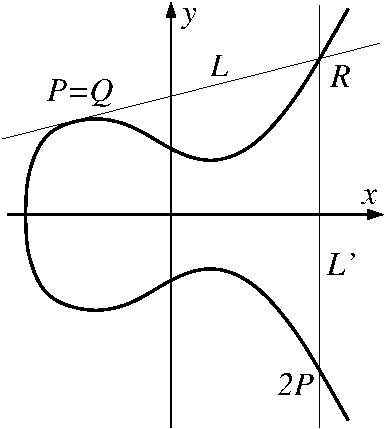
\includegraphics[scale=1.08]{figures/ec-mult2}
\caption{Verdoppelung eines Punktes} 
\vspace{\floatsep}
\vskip +20 pt
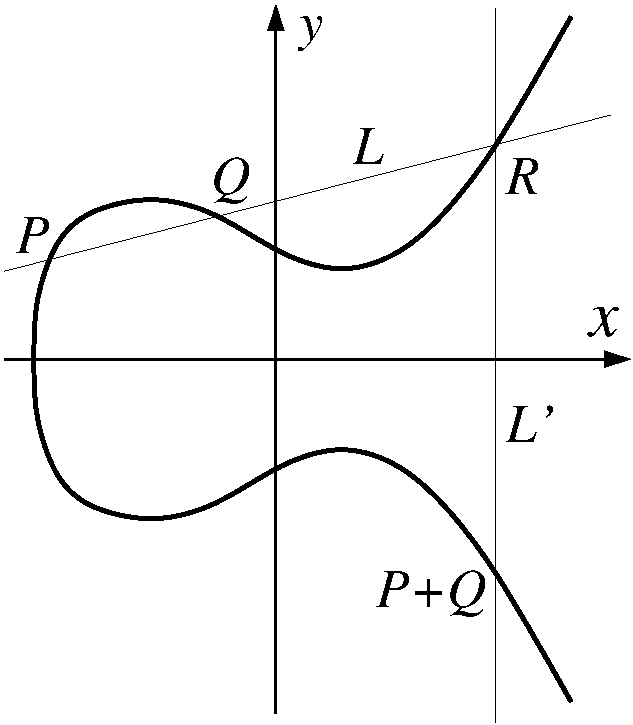
\includegraphics[scale=0.65]{figures/ec-add}
\caption{Addition zweier verschiedener Punkte} % \footnotemark }
\end{center}
\end{figure}
% \addtocounter{footnote}{0}\footnotetext{Der Punkt $O$ kann nicht in der affinen Ebene dargestellt werden.}
\enlargethispage{+20pt}
\newpage
Zu beachten ist, dass man
${\bf E}$ folgende Bedeutungen zuordnen kann:
\begin{itemize}
   \item die Menge ${\bf E}$ der L"osungspaare $(x,y)$ einer Gleichung inklusive dem Punkt $O$ %\\[-20 pt]
   \item die Gruppe ${\bf E}$ (mit der Verkn"upfung \glqq Addition von $(x_1,y_1)$ und $(x_2,y_2)$\grqq) %\\[-20 pt]
   \item die Elliptische Kurve ${\bf E}$ (die eigentlich dasselbe wie die Gruppe ${\bf E}$ ist) %\\[-20pt]
 \end{itemize}

Da diese Bezeichnungen eigentlich alle dasselbe meinen, ist eine Unterscheidung "uber die genaue Bedeutung nur
selten n"otig.

F"ur die Kryptographie ist die Tatsache von Bedeutung, dass es f"ur sehr gro"se Zahlen extrem schwierig zu
sein scheint, aus einem gegebenem Punkt $Q$ auf einer Elliptischen Kurve festzustellen, welche beiden
Punkte addiert werden m"ussen, um $Q$ zu erhalten.

F"ur gro"se Zahlen $a, b$ und $p$ ($p$ ist zum Beispiel
mehr als $160$ Bit lang) ist der Computer ohne weiteres in der Lage, sehr schnell (in wenigen
Bruchteilen einer Sekunden) den Punkt $P$  $m$ mal hintereinander zu addieren, also den Punkt
$P + P + \cdots + P = Q$ ($m$ Summanden $P$) zu bestimmen. Statt $P + P + \cdots + P = Q$ ($m$ Summanden $P$)
schreibt man auch $mP = Q$. Hat man einen Punkt $P$ und einen Punkt $Q$, die beide auf der gleichen
Elliptischen Kurve liegen, ist allerdings kein Verfahren bekannt, das es erm"oglicht --- in
akzeptabler Zeit --- diejenige Zahl $m$ zu bestimmen (falls es diese "uberhaupt gibt), mit der $mP = Q$ gilt.
Dies wird als das \glqq Diskrete Logarithmus Problem "uber Elliptischen Kurven\grqq\ bezeichnet
(auch ECDLP\index{ECDLP} - Elliptic Curve Discrete Logarithm Problem - abgek"urzt).
\vskip +5 pt

Es ist zu beachten, dass nicht alle Elliptischen Kurven gleich sicher sind. Das bedeutet, dass man bei der
Definition einer Kurve auf die Wahl der Parameter $a$ und $b$ achten muss. Denn f"ur bestimmte Klassen von
Elliptischen Kurven ist es m"oglich, das ECDLP leichter zu l"osen als im allgemeinen Fall. Kryptographisch
ungeeignete Elliptische Kurven sind die sogenannten {\em anormalen} Kurven (das sind Kurven "uber ${\mathbb Z}_p$,
f"ur die die Menge ${\bf E}$ genau $p$ Elemente hat) und die {\em supersingul"aren} Kurven (das sind Kurven, f"ur die man das
Berechnen des ECDLP auf das Berechnen des \glqq normalen\grqq\ Diskreten Logarithmus in anderen endlichen K"orper
reduzieren, d.h. vereinfachen, kann). Daher gibt es kryptographisch gute und schlechte Kurven. Allerdings
kann man f"ur gegebene Parameter $a$ und $b$ mit etwas Aufwand feststellen, ob die resultierende Elliptische
Kurve kryptographisch brauchbar ist oder nicht. Die in der Kryptographie eingesetzten Kurven werden meist
von Fachleuten zur Verf"ugung gestellt. Sie gew"ahrleisten, dass die von ihnen als sicher eingestuften
Elliptischen Kurven den aktuellen Sicherheitsanforderungen gen"ugen.
\vskip +5 pt

Bei sicheren Kurven wird haupts"achlich
durch den Parameter $p$ bestimmt, wie lange es dauert, das ECDLP auf dieser Kurve zu l"osen. Je gr"o"ser der
Parameter $p$ ist, desto l"anger nimmt das L"osen des Problems in Anspruch. Von Fachleuten wird eine Bitl"ange
von "uber $200$ Bit f"ur den Parameter $p$ empfohlen. Hier wird deutlich, warum die Elliptischen Kurven so
interessant f"ur die Kryptographie sind. Denn der Parameter $p$ bestimmt auch den
Signatur-/Verschl"usselungsaufwand, der aufgewendet werden muss, wenn mit Elliptischen Kurven
Kryptographie betrieben wird. Die Dauer einer Schl"usselpaar-Erzeugung ist ebenfalls von
$p$ abh"angig. Daher sind kleine Werte (wenige Bits) w"unschenswert (m"oglichst schnelle Laufzeiten der Verfahren);
allerdings muss die geforderte Sicherheit dabei eingehalten werden. Mit einer L"ange von zum Beispiel $200$ Bit
f"ur $p$ ist eine {\em gute} Elliptische Kurve genau so sicher wie ein \index{RSA!Modul} RSA-Modul von "uber $1024$ Bit L"ange
(zumindest nach dem heutigen Forschungstand). Der Grund daf"ur ist, dass die schnellsten Algorithmen zum
L"osen des {\em Elliptische Kurven Diskreter Logarithmus} Problems eine exponentielle Laufzeit haben --- im
Gegensatz zu den subexponentiellen Laufzeiten, die die zur Zeit besten Faktorisierungsalgorithmen haben
(Zahlk"orpersieb, Quadratisches Sieb oder Faktorisieren mit Elliptischen Kurven). Daher m"ussen die
Parameter von Kryptoverfahren, die auf dem Problem {\em Faktorisieren von ganzen Zahlen} beruhen, gr"o"ser sein als
die Parameter von Kryptoverfahren, die auf dem ECDL-Problem basieren.

% --------------------------------------------------------------------------------------------------------------------
\subsubsection{Digitale Signaturen mit Elliptischen Kurven}

\begin{sloppypar}
  Das {\em Elliptische Kurven Diskreter Logarithmus
    Problem}\index{Logarithmusproblem} (ECDLP) \index{ECDLP} ist die
  Grundlage f"ur die Elliptische-Kurven-Kryptographie. Ausgehend von
  dieser Grundlage gibt es verschiedene Signaturverfahren.  Sie haben
  gemeinsam, wie sie die folgenden "offentlichen Parameter benutzen und wie
  damit der geheime und der "offentliche Schl"ussel erzeugt werden:
\end{sloppypar}
\begin{itemize}
    \item Die Parameter der Elliptischen Kurve {\bf E}, das hei"st eine Primzahl $p$, die festlegt,
          "uber welchem K"orper ${\mathbb Z}_p$ die Elliptische Kurve ${\bf E}$ definiert ist, sowie die beiden
          Zahlen $a$ und $b$ aus ${\mathbb Z}_p$.
    \item Ein Punkt $G=(x,y)$, der auf der Elliptischen Kurve ${\bf E}$ liegt.
    \item Eine Primzahl $r < p$, f"ur die gilt $rG=O$ (also $r$ mal $G$ addiert ergibt das neutrale Element der
          Gruppe ${\bf E}$) und $r$ ist ein Teiler von $\#{\bf E}$ (mit $\# {\bf E}$ ist die Anzahl der Elemente in der
          Menge ${\bf E}$ gemeint). Der Punkt $G$ hat also die Ordnung $r$ und ist der Generator einer
          zyklischen Untergruppe von ${\bf E}$ mit der Ordnung $r$.
    \item Die Zahl $k = \#{\bf E}/r$ ($k$ ist der sogenannte {\em Kofaktor}).
\end{itemize}
Die eben genannten Parameter $a, b, p, G, r$ und $k$ bezeichnet man als \index{Domain-Parameter} {\em Domain}-Para\-meter. Durch sie wird
festgelegt, auf welcher Elliptischen Kurve ${\bf E}$ und in welcher zyklischen Untergruppe von ${\bf E}$ ein
Signaturverfahren \glqq eingesetzt\grqq\ wurde.

Der geheime Schl"ussel $s$ des Signaturerstellers ist eine (zuf"allige\index{Zufall}) ganze Zahl $s$ aus dem
Intervall $[1, r-1]$. Der "offentliche Schl"ussel des Signaturerstellers ist ein Punkt $W=(x,y)$ auf der
Elliptischen Kurve ${\bf E}$. "Offentlicher Schl"ussel $W$ und geheimer Schl"ussel $s$ h"angen wie folgt voneinander ab:
$W = sG$. Das hei"st durch die Domain-Parameter (insbesondere $G$) und den geheimen Schl"ussel $s$
wird der "offentliche Schl"ussel $W$ berechnet (durch $s$-malige Addition von $G$ auf ${\bf E}$). Hier wird ganz
offensichtlich von dem ECDLP Gebrauch gemacht: Kennt jemand $W$ und $G$
(sowie die anderen benutzten Domain-Para\-meter), so ist es schwierig, daraus $s$ zu berechnen
(f"ur richtig gew"ahlte Parameter scheint dies zur Zeit praktisch unm"oglich zu sein).

Um eine Signatur zu verifizieren, muss dem Empf"anger der Signatur folgendes bekannt sein:
\begin{enumerate}
   \item das eingesetzte Signaturverfahren,
   \item die eingesetzte Hashfunktion,
   \item die zum Signieren benutzten Domain-Parameter und
   \item der "offentliche Schl"ussel $W$ des Signaturerstellers.
\end{enumerate}


% --------------------------------------------------------------------------------------------------------------------------
\subsubsection{Faktorisieren mit Elliptischen Kurven}
\hypertarget{faktell}{}

Es gibt Faktorisierungsalgorithmen, die auf Elliptischen Kurven \index{Faktorisierungsalgorithmen}
basieren\footnote{Im Jahr 1987 stellte H.W. Lenstra\index{Lenstra 1987}
einen Faktorisierungsalgorithmus vor, der auf Elliptischen Kurven basiert 
(Siehe \cite{Lenstra1987}). Die aktuell gr"o"ste mit Elliptischen Kurven faktorisierte Zahl  
ist die 55 Dezimalstellen lange Zahl $629^{59}-1$, sie wurde am 6. Oktober 2001 von M. Izumi gefunden (Siehe \hyperlink{Lenstra2}{ECMNET}\index{ECMNET}).}. 
Genauer gesagt, machen sich diese Verfahren zunutze, dass man auch "uber ${\mathbb Z}_n$ ($n$ zusammengesetzte Zahl)
Elliptische Kurven definieren kann. Elliptische Kurven "uber ${\mathbb Z}_n$ bilden keine Gruppe, da es nicht zu jedem 
Punkt auf solchen Elliptischen Kurven einen inversen Punkt geben muss. Dies h"angt damit zusammen, dass es -- falls $n$ 
eine zusammengesetzte Zahl ist -- in ${\mathbb Z}_n$ Elemente gibt, die kein Inverses bez"uglich der Multiplikation
modulo $n$ haben. Um zwei Punkte auf einer Elliptischen Kurve "uber ${\mathbb Z}_n$ zu addieren, kann
prinzipiell genauso gerechnet werden wie auf Elliptischen Kurven "uber ${\mathbb Z}_p$. Eine Addition von zwei
Punkten (auf einer Elliptischen Kurve "uber ${\mathbb Z}_n$) scheitert aber genau dann, wenn man einen Teiler
von $n$ gefunden hat. Der Grund daf"ur ist, dass das Verfahren zum Addieren von Punkten auf Elliptischen
Kurven Elemente in ${\mathbb Z}_n$ ermittelt und zu diesen Elementen die inversen Elemente (bez"uglich der
Multiplikation modulo $n$) in ${\mathbb Z}_n$ berechnet. Dazu wird der erweiterte \index{Euklidscher Algorithmus} Euklidsche Algorithmus benutzt.
Ergibt sich nun bei der Addition zweier Punkte (die auf einer Elliptischen Kurve "uber ${\mathbb Z}_n$ liegen) ein
Element aus ${\mathbb Z}_n$, das kein inverses Element in ${\mathbb Z}_n$ hat, so gibt der erweiterte Euklidsche Algorithmus\index{Euklidscher Algorithmus!erweiterter}
einen echten Teiler von $n$ aus.

Das Faktorisieren mit Elliptischen Kurven funktioniert somit prinzipiell so: Man w"ahlt zuf"allige Kurven
"uber ${\mathbb Z}_n$, sowie zuf"allig irgendwelche Punkte (die auf diesen Kurve liegen) und addiert diese; dabei
bekommt man wieder Punkte, die auf der Kurve liegen oder findet einen Teiler von $n$. Die
Faktorisierungsalgorithmen auf Basis von Elliptischen Kurven arbeiten also probabilistisch.
Durch die M"oglichkeit, sehr viele Elliptische Kurven "uber ${\mathbb Z}_n$ zu definieren, kann man die
Wahrscheinlichkeit erh"ohen, zwei Punkte zu finden, bei deren Addition ein Teiler von $n$ gefunden wird.
Daher eigenen sich diese Verfahren auch sehr gut f"ur Parallelisierung.

% ---------------------------------------------------------------------------------------------------------------------
\subsection{Implementierung Elliptische Kurven}

CrypTool\index{CrypTool} bietet bei der Funktion f"ur digitale Signaturen auch Elliptische Kurven an.

Implementiert sind die Basisalgorithmen f"ur Gruppenoperationen, f"ur das Erzeugen von Elliptischen
Kurven und f"ur das Ein- und Auslesen von Parametern f"ur Elliptische Kurven "uber endlichen
K"orpern mit $p$ ($p$ prim) Elementen. Die Implementierung erfolgte in ANSI C und richtete sich
nach dem Entwurf Nr.8 der Arbeitsgruppe IEEE P1363 {\em Standard Specifications for Public Key Cryptography}

{\href{http://grouper.ieee.org/groups/1363}{\texttt{http://grouper.ieee.org/groups/1363}}}.

Implementiert sind die kryptographischen Primitive zur Signaturerzeugung und Signaturverifikation f"ur
die auf Elliptischen Kurven basierenden Varianten von Nyberg-Rueppel-Signaturen und \index{DSA} DSA-Signaturen
(nach Entwurf Nr.8 der Arbeitsgruppe IEEE P1363). Dies erfolgte in Zusammenarbeit mit der Secude
GmbH --- und unter Benutzung der obigen Bibliothek und des Secude SDK.
\index{Secude GmbH}


%--------------------------------------------------------------------
\newpage
\begin{thebibliography}{99999}
\addcontentsline{toc}{subsection}{Literaturverzeichnis}

\bibitem[Lenstra1987]{Lenstra1987} H.W. Lenstra\\ \index{Lenstra 1987}
                Factoring integers with elliptic curves, 
		Annals of Mathematics 126, pp. 649-673, 1987.

\end{thebibliography}


%--------------------------------------------------------------------
%\newpage
\section*{Web-Links}\addcontentsline{toc}{subsection}{Web-Links}

\begin{enumerate}
   \item Online-Tutorial "uber Elliptische Kurven der Firma Certicom
         \index{Certicom}\\
         \href{http://www.certicom.com/resources/ecc_tutorial/ecc_tutorial.html}         {\texttt{http://www.certicom.com/resources/ecc\_tutorial/ecc\_tutorial.html}}

   \item Arbeitsgruppe IEEE P1363
         \href{http://grouper.ieee.org/groups/1363}{\texttt{http://grouper.ieee.org/groups/1363}}
        
   \item \hypertarget{Lenstra2} Eine informative Seite zum Faktorisieren 
         mit Elliptischen Kurven. \\
        \href{http://www.loria.fr/~zimmerma/records/ecmnet.html}
	{\texttt{http://www.loria.fr/\~{}zimmerma/records/ecmnet.html}} \\
        Dort findet man Literatur zum Thema Faktorisieren mit Elliptischen
	Kurven sowie Links zu anderen Seiten.

\end{enumerate}

% Local Variables:
% TeX-master: "../script-de.tex"
% End:
